\documentclass{article}\usepackage[]{graphicx}\usepackage[]{color}
% maxwidth is the original width if it is less than linewidth
% otherwise use linewidth (to make sure the graphics do not exceed the margin)
\makeatletter
\def\maxwidth{ %
  \ifdim\Gin@nat@width>\linewidth
    \linewidth
  \else
    \Gin@nat@width
  \fi
}
\makeatother

\definecolor{fgcolor}{rgb}{0.345, 0.345, 0.345}
\newcommand{\hlnum}[1]{\textcolor[rgb]{0.686,0.059,0.569}{#1}}%
\newcommand{\hlstr}[1]{\textcolor[rgb]{0.192,0.494,0.8}{#1}}%
\newcommand{\hlcom}[1]{\textcolor[rgb]{0.678,0.584,0.686}{\textit{#1}}}%
\newcommand{\hlopt}[1]{\textcolor[rgb]{0,0,0}{#1}}%
\newcommand{\hlstd}[1]{\textcolor[rgb]{0.345,0.345,0.345}{#1}}%
\newcommand{\hlkwa}[1]{\textcolor[rgb]{0.161,0.373,0.58}{\textbf{#1}}}%
\newcommand{\hlkwb}[1]{\textcolor[rgb]{0.69,0.353,0.396}{#1}}%
\newcommand{\hlkwc}[1]{\textcolor[rgb]{0.333,0.667,0.333}{#1}}%
\newcommand{\hlkwd}[1]{\textcolor[rgb]{0.737,0.353,0.396}{\textbf{#1}}}%
\let\hlipl\hlkwb

\usepackage{framed}
\makeatletter
\newenvironment{kframe}{%
 \def\at@end@of@kframe{}%
 \ifinner\ifhmode%
  \def\at@end@of@kframe{\end{minipage}}%
  \begin{minipage}{\columnwidth}%
 \fi\fi%
 \def\FrameCommand##1{\hskip\@totalleftmargin \hskip-\fboxsep
 \colorbox{shadecolor}{##1}\hskip-\fboxsep
     % There is no \\@totalrightmargin, so:
     \hskip-\linewidth \hskip-\@totalleftmargin \hskip\columnwidth}%
 \MakeFramed {\advance\hsize-\width
   \@totalleftmargin\z@ \linewidth\hsize
   \@setminipage}}%
 {\par\unskip\endMakeFramed%
 \at@end@of@kframe}
\makeatother

\definecolor{shadecolor}{rgb}{.97, .97, .97}
\definecolor{messagecolor}{rgb}{0, 0, 0}
\definecolor{warningcolor}{rgb}{1, 0, 1}
\definecolor{errorcolor}{rgb}{1, 0, 0}
\newenvironment{knitrout}{}{} % an empty environment to be redefined in TeX

\usepackage{alltt}
\usepackage{natbib}
\usepackage{hyperref}
\usepackage{graphicx}
\usepackage{subcaption}
\usepackage{amsmath}
\bibliographystyle{apalike}

\title{SIR Model with Testing and Isolation Mechanisms}
\IfFileExists{upquote.sty}{\usepackage{upquote}}{}
\begin{document}
\maketitle

% %%%%%%%
\section{Method}

\subsection{model and parameters}
\begin{itemize}
\item $\Lambda$: force of infection defined as $$\Lambda=\beta \frac{(I_u+\eta_w I_n+\eta_w I_p+ \eta_t I_t)}{N_0},$$ where $\beta$ is transmission rate, $\eta_w$ and $\eta_t$ are the isolation parameters for awaiting and reported individuals, respectively. We assume that $\eta_t<\eta_w$, i.e., the awaiting individuals for test results have a higher transmission probability than the reported individuals.
\item $\omega$: the rate of *onward flow* from the awaiting positive compartment, $p$, to reported/tested compartment, $\rho$, or from awaiting negative compartment, $n$, back to $u$.  It has units of $1/time$.
\item $\gamma$: recovery rate ($1/time$).
\item $\rho$: per capita testing intensity across the whole population ($1/time$).
\item $W$: weighted number of people available for tests, defined as $W = W_S S_u + W_I I_u + W_R R_u$.
\item $\sigma$: scaling parameter for testing defined as $\sigma = \frac{\rho N_0}{W}$.
\item $F_Z$: Weighted testing rate defined as $F_Z=\sigma W_Z$. That is, $F_S = \sigma W_S$, $F_I=\sigma W_I$ and $F_R = \sigma W_R$.
\end{itemize}

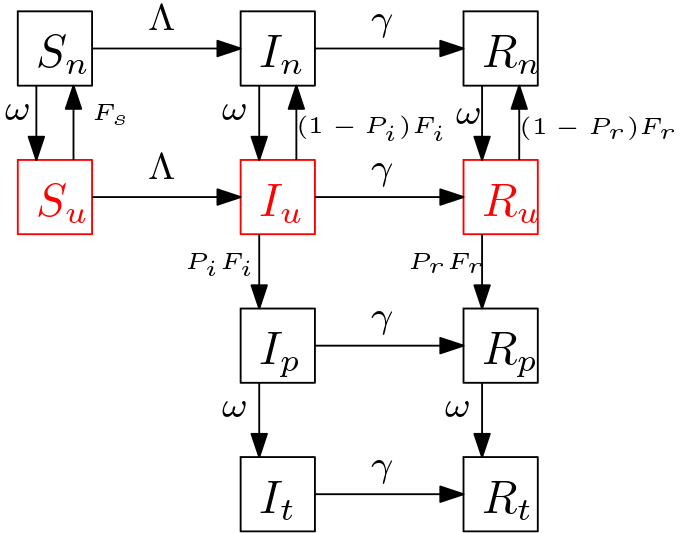
\includegraphics[width=\linewidth]{../pix/sir_comp2.png}

The model is

\begin{align}
\label{mod:1}
 d S_u/dt &= -\Lambda S_u - F_S S_u + \omega S_n \\
 d S_n/dt &= -\Lambda S_n + F_S S_u - \omega S_n \\
 d I_u/dt &= \Lambda S_u - F_I I_u + \omega I_n  - \gamma I_u  \\
 d I_n/dt &= \Lambda S_n + (1-p_I) F_I I_u - \omega I_n -\gamma I_n \\
 d I_p/dt &= p_I F_I I_u - \omega I_p -\gamma I_p \\
 d I_t/dt &= \omega I_p - \gamma I_t  \\
 d R_u/dt &= \gamma I_u - F_R R_u + \omega R_n \\
 d R_n/dt &= \gamma I_n + (1-p_R) F_R R_u - \omega R_n  \\
 d R_p/dt &= \gamma I_p + p_R F_R R_u  - \omega R_p  \\
 d R_t/dt&= \gamma I_t + \omega R_p  \\
 dN/dt &= \omega (S_n + I_n + R_n)   \\
 dP/dt &= \omega(I_p + R_p).
\end{align}

% %%%%%%%
\section{Results}

\newpage
\begin{figure}
\centering
\begin{subfigure}[t]{.45\textwidth}
\centering
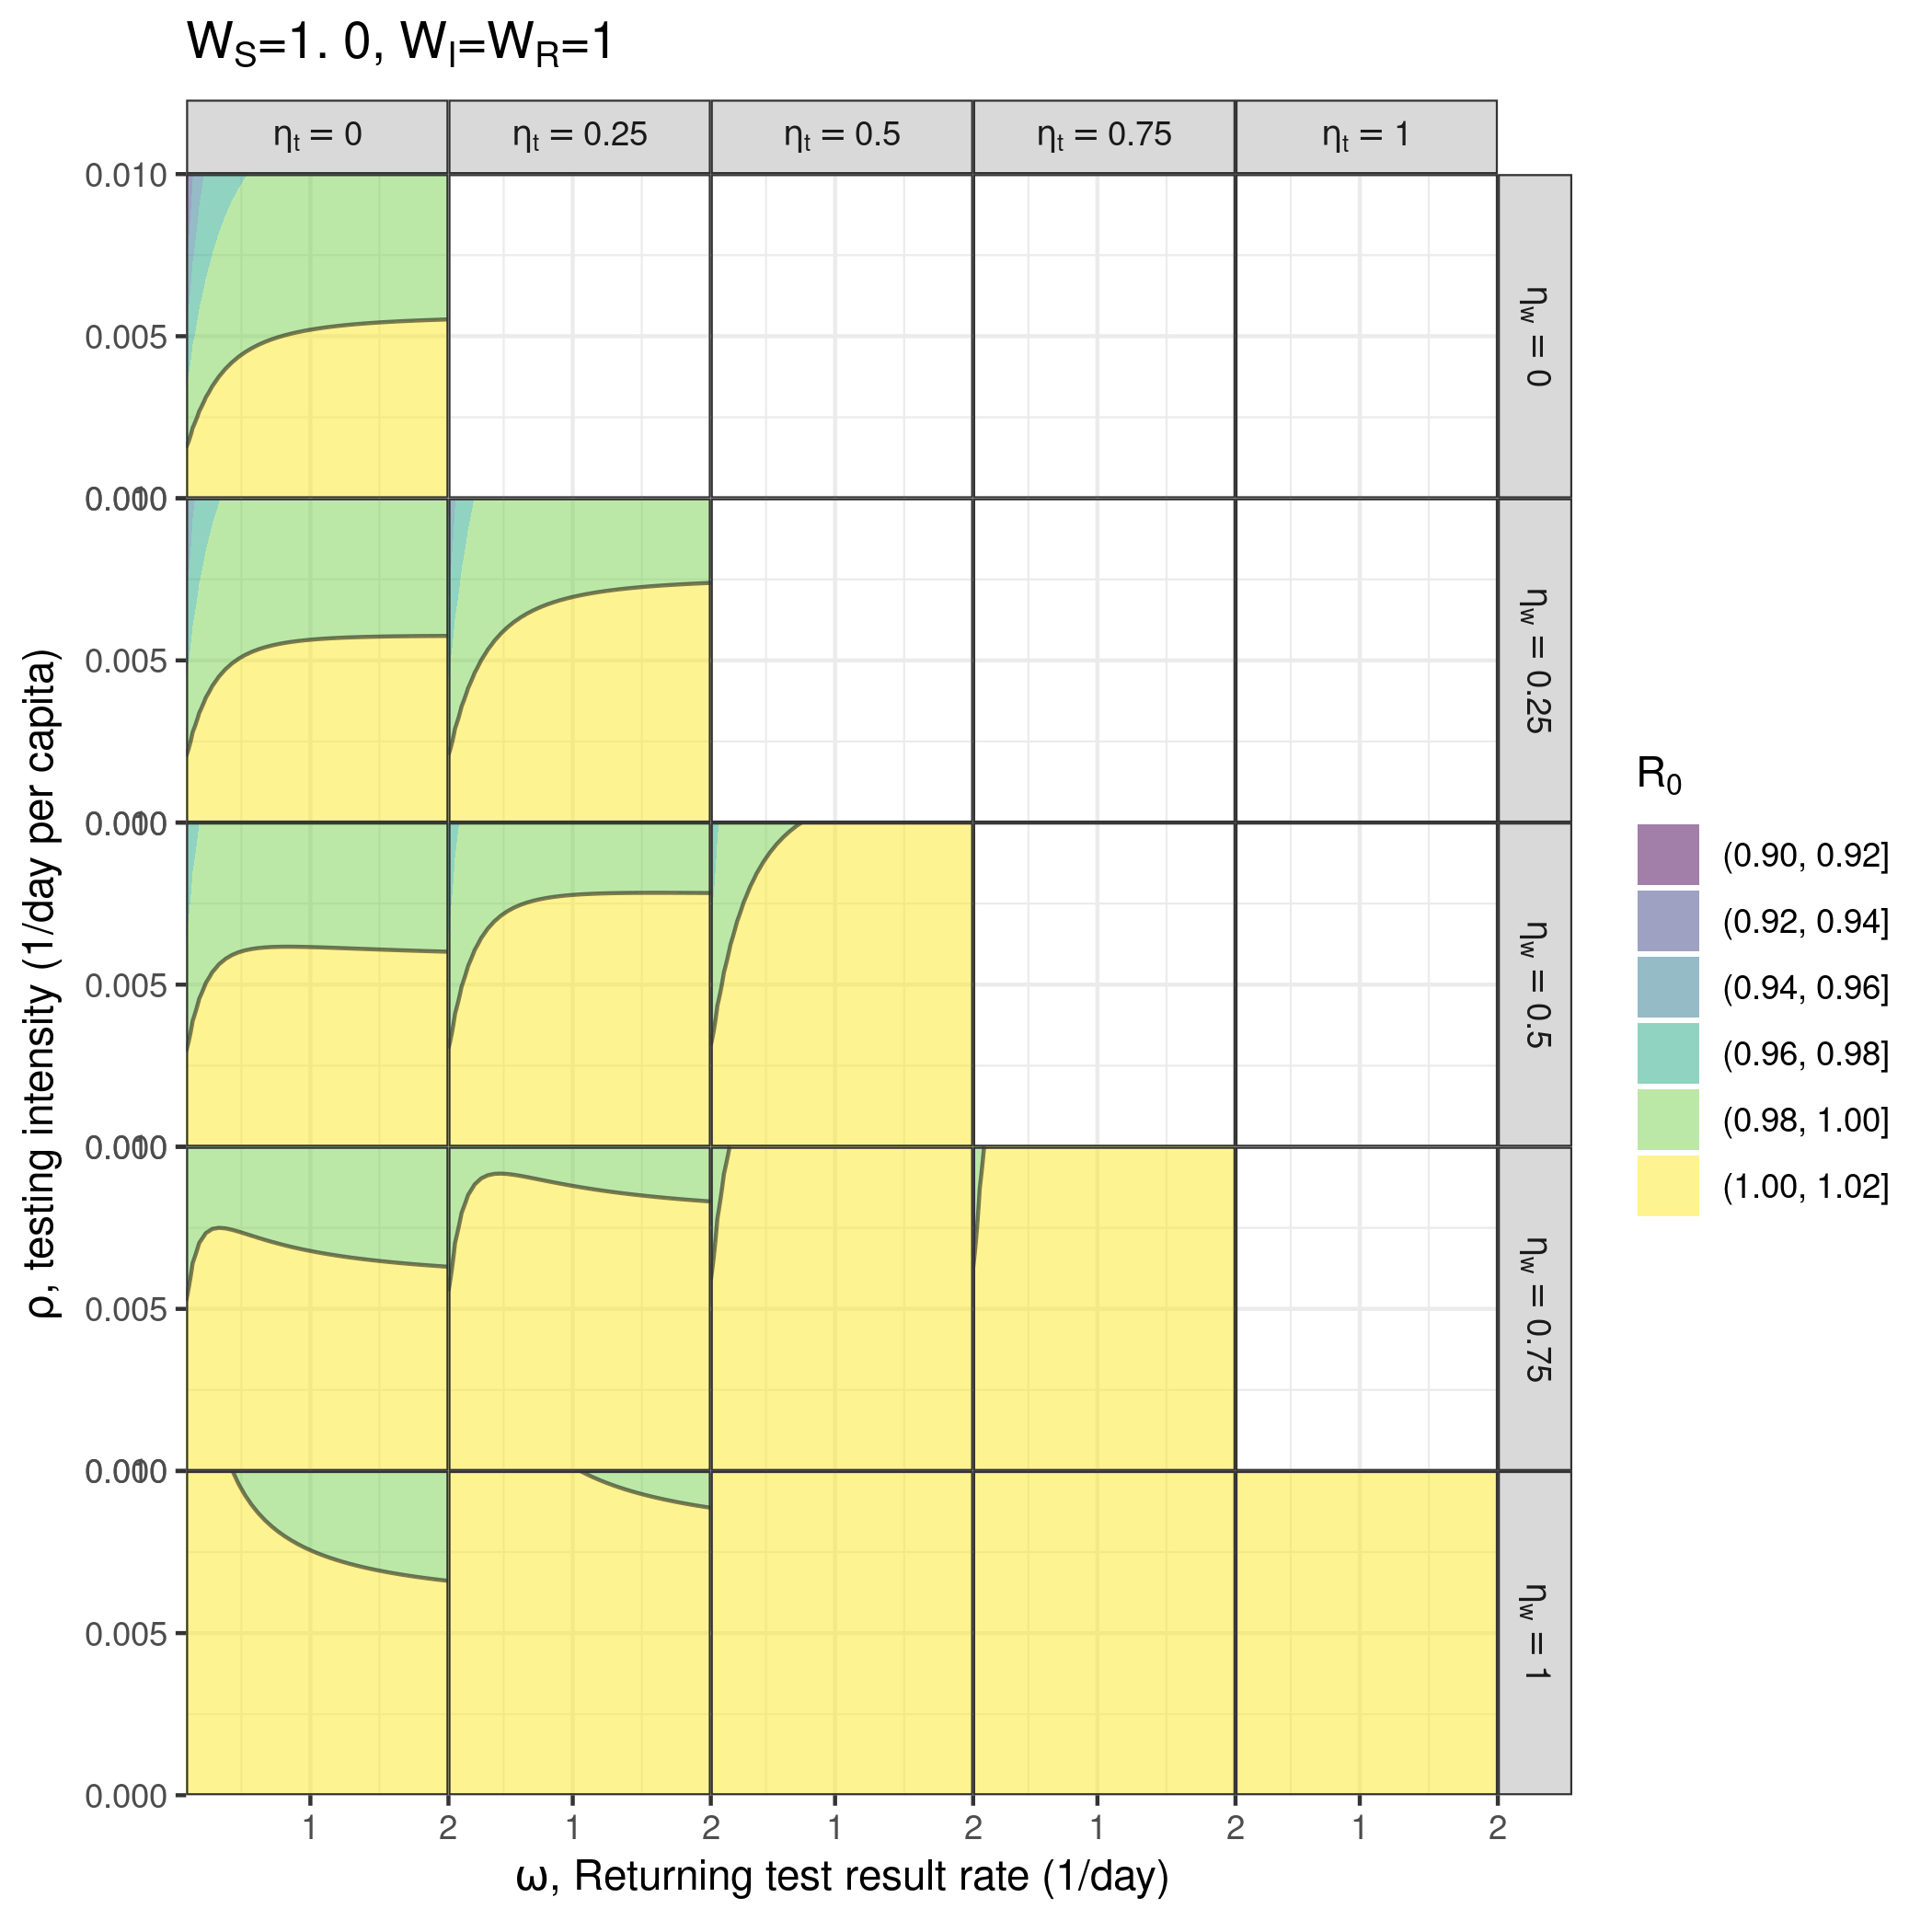
\includegraphics[width=\linewidth]{../pix/R0contour_random.png}
        \caption{}\label{fig:fig_a}
\end{subfigure}
%
\begin{subfigure}[t]{.45\textwidth}
\centering
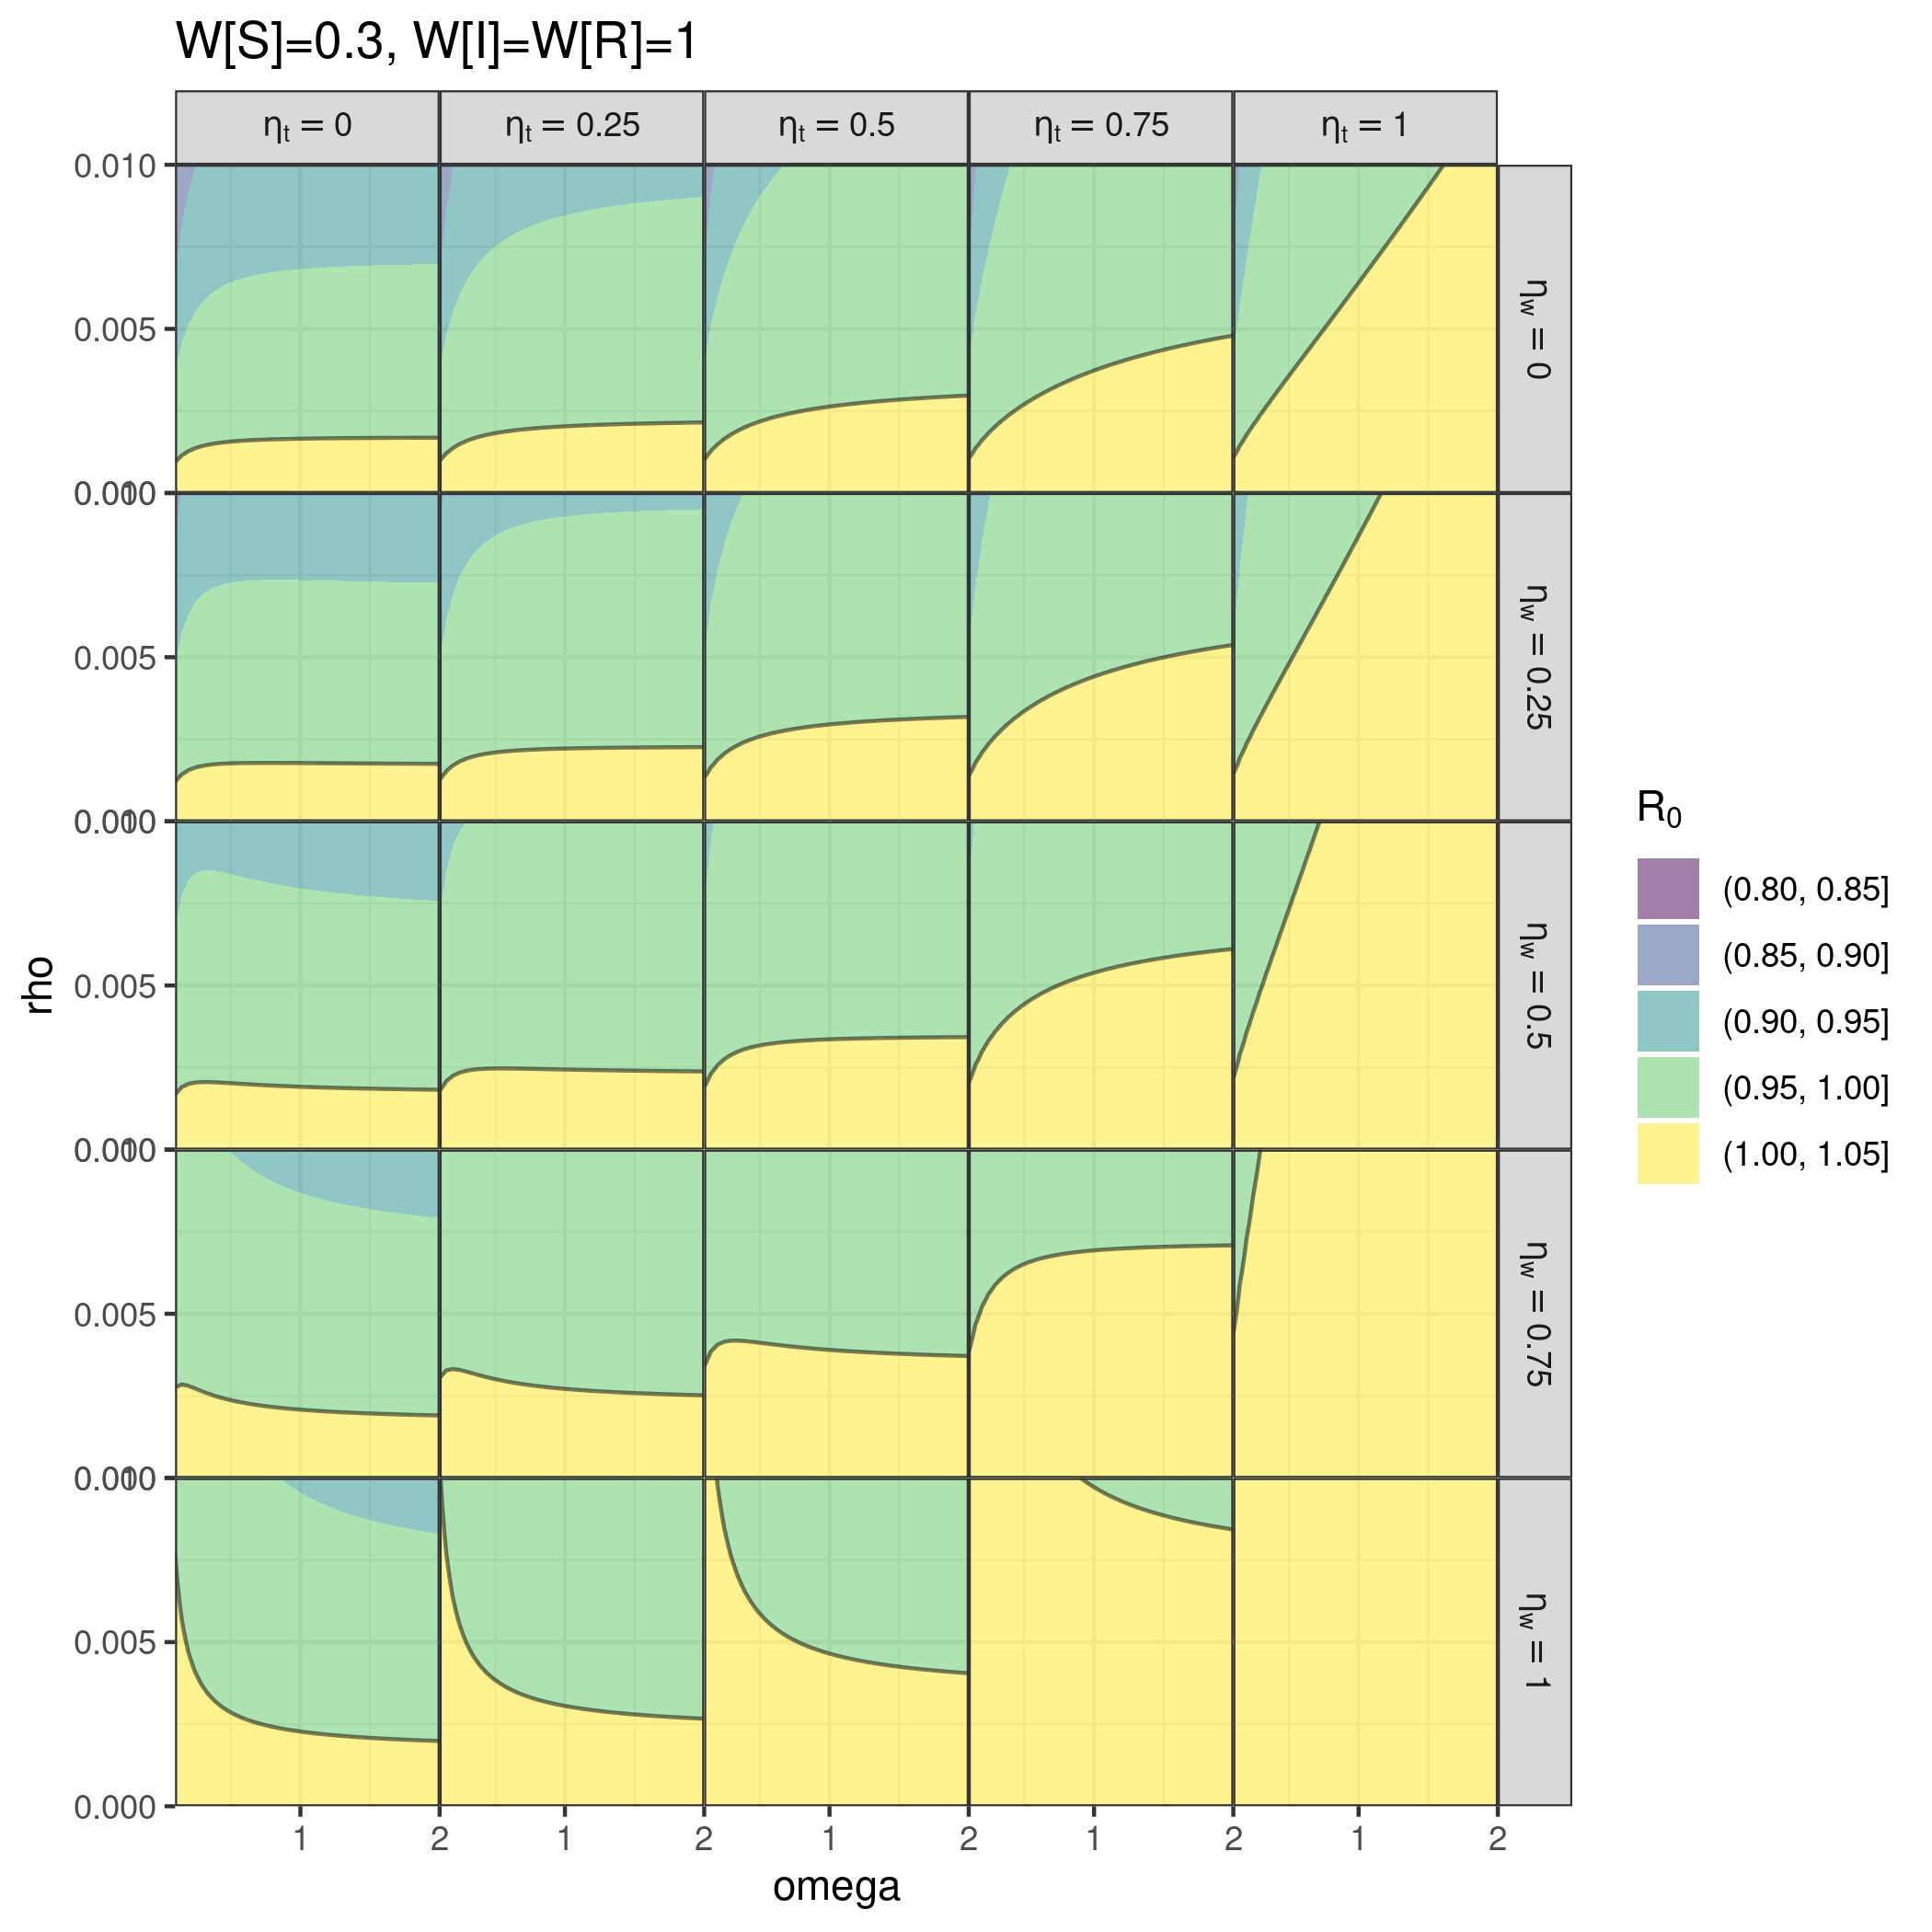
\includegraphics[width=\linewidth]{../pix/R0contour_TTI.png}
\caption{}\label{fig:fig_b}
\end{subfigure}
\end{figure}

\begin{figure}
\centering
\begin{subfigure}[t]{.45\textwidth}
\centering
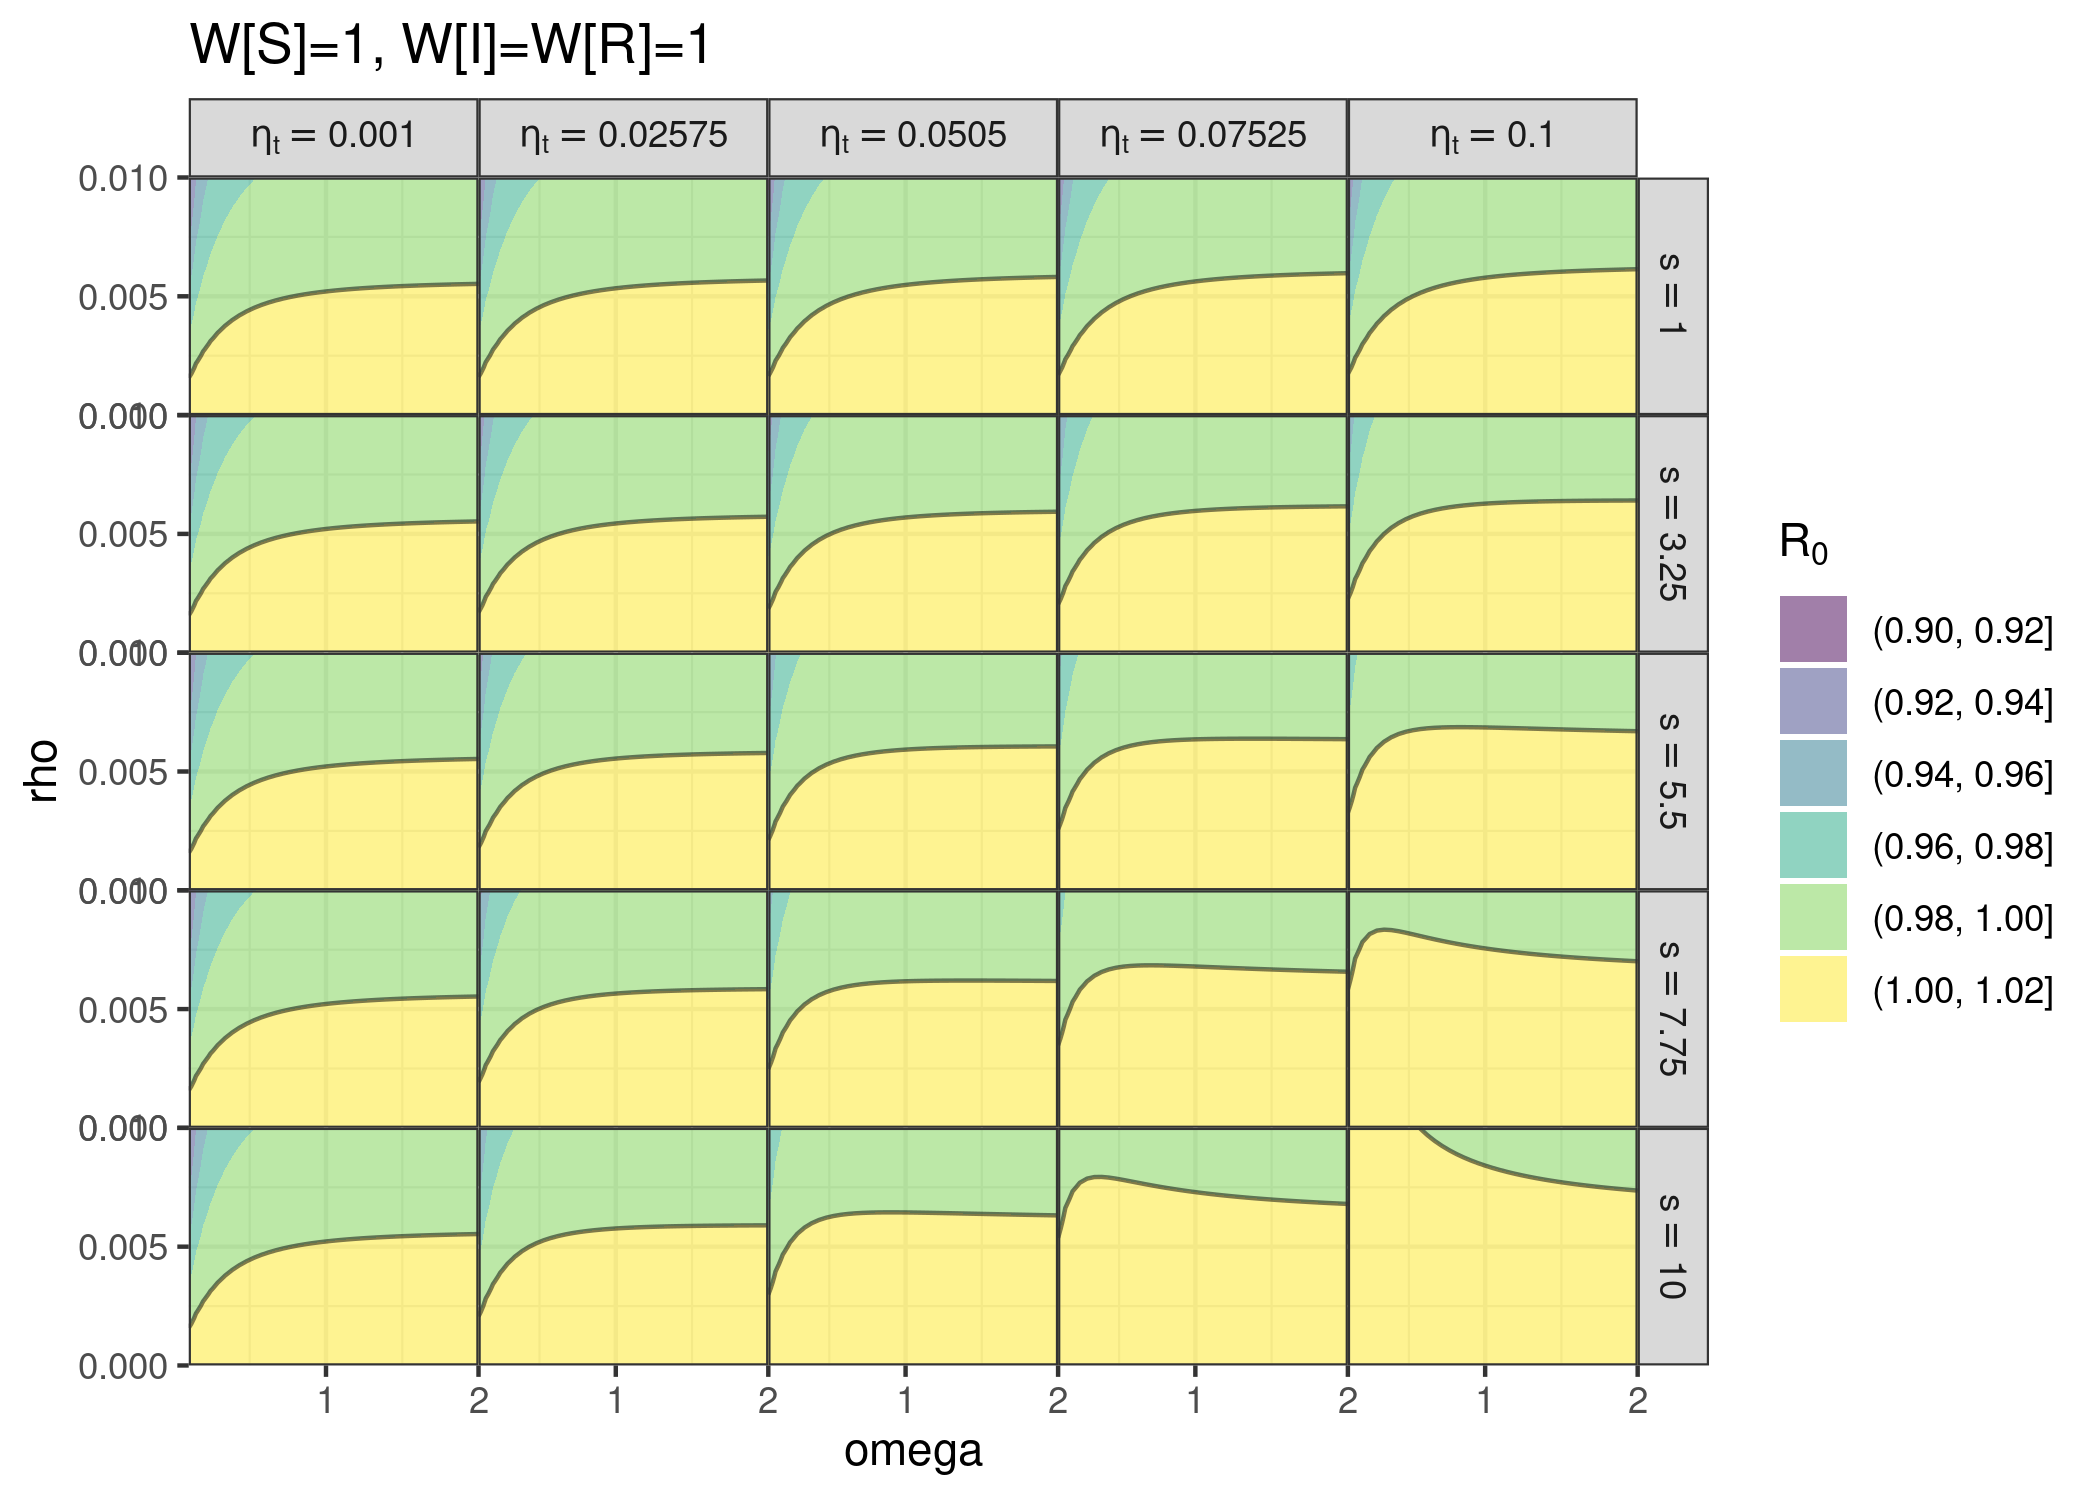
\includegraphics[width=\linewidth]{../pix/R0contour_random_s.png}
        \caption{}\label{fig:fig_a}
\end{subfigure}
%
\begin{subfigure}[t]{.45\textwidth}
\centering
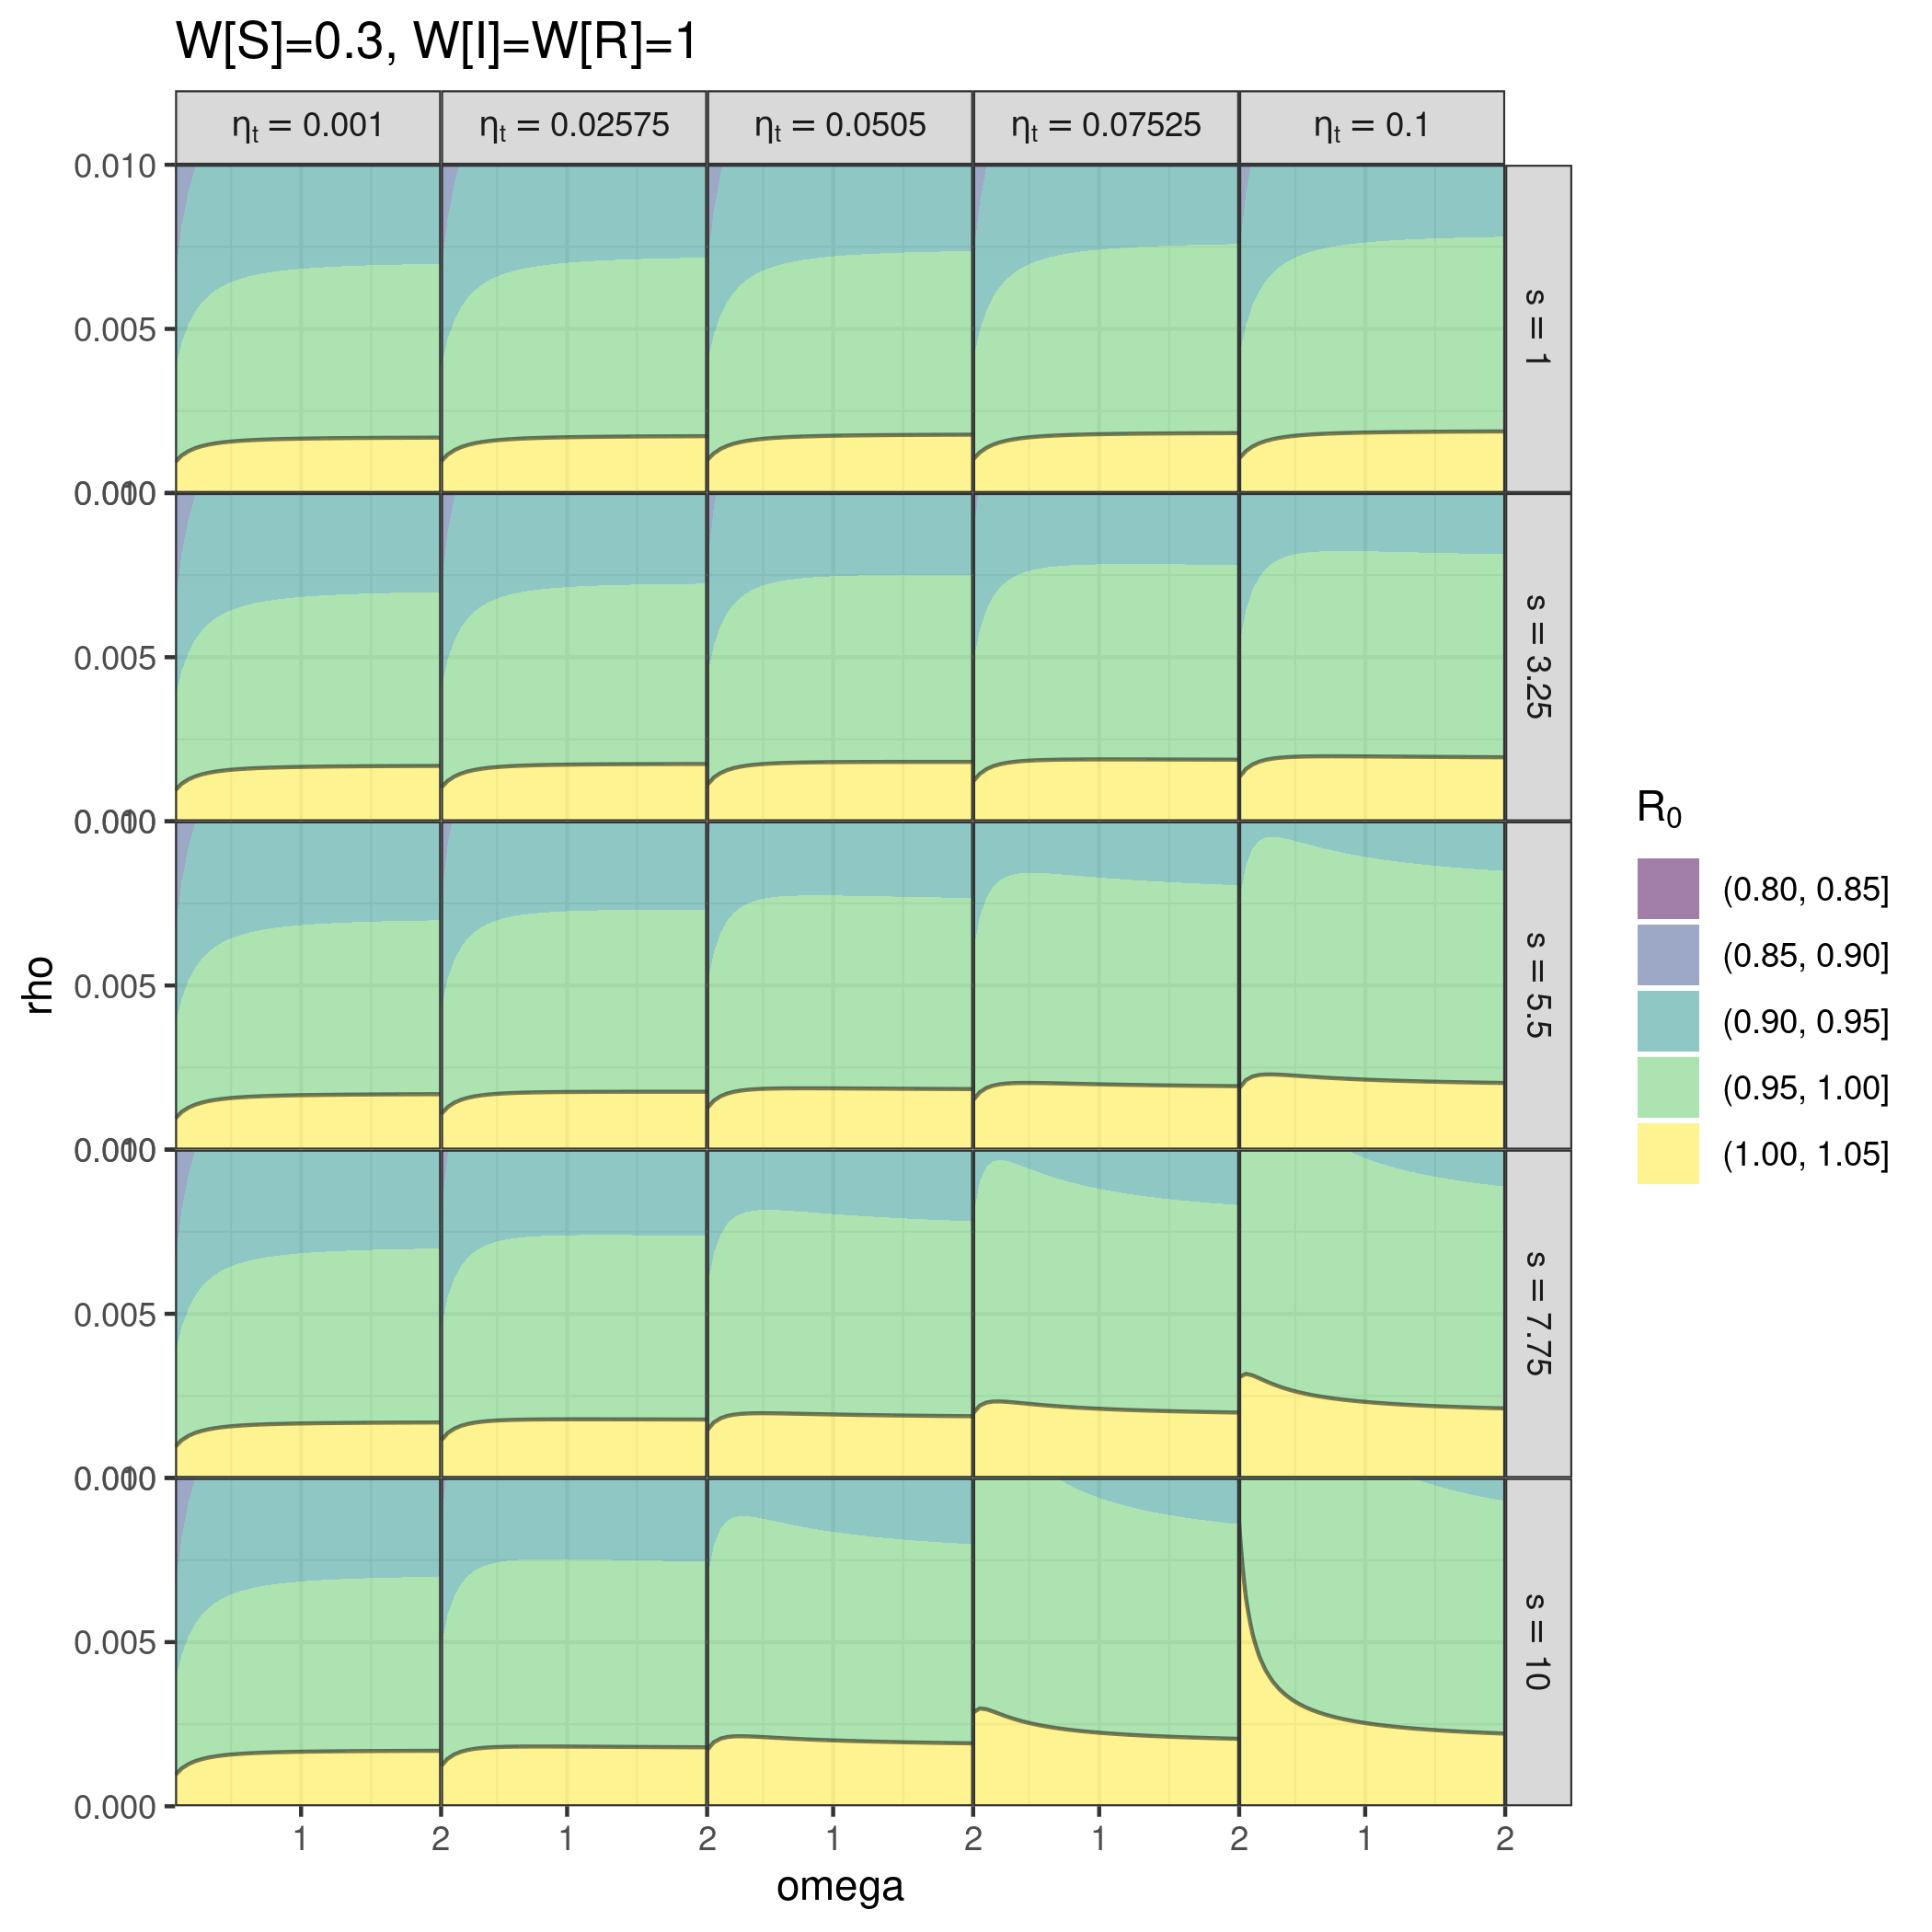
\includegraphics[width=\linewidth]{../pix/R0contour_TTI_s.png}
\caption{}\label{fig:fig_b}
\end{subfigure}
\end{figure}

**Insights from the R0-contour plots**

1. TTI requires lower testing rate than random testing to achieve $R_0=1$.

2. When random testing regime is applied, $W_S=W_I=W_R$,

(i) in the case of perfect isolation of the reported individuals, $\eta_t=0$, the followings are inferred (see the first few columns of the panel plot); 
 - variations of the $\eta_w$ has a negligible effect on the critical testing.
 - for low $\omega$, $R_0$ increases as $\omega$ increases but saturates. This means that when the reporting process is very very slow, increasing the speed of the reporting causes higher $R_0$. Maybe because more people will move to $I_u$ [?, not very sure here.]
 
 (ii) in case of the non-perfect isolation (see the last column), when $\eta_w$ increases (more awaiting people follow the isolation rules) faster reporting reduces $R_0$.  
Note that it is sensible to expect that $\partial{R_0}/\partial{\omega}<0$. Here we showed that this can be less true. 

3. When TTI regime is applied,


% %%%%%%%
\section{Thoughts/Objectives}



\begin{enumerate}
\item 
\begin{itemize}
\item analysis of the basic SIR model with testing: analytical results as far as possible, supplemented by numerical results as necessary/for illustration. Heuristic explanations/insights of what we learn from this.
\item Maybe?? order-of-magnitude/back-of-the-envelope calculations of the magnitudes of testing and isolation necessary. (However, the model may be too simplified for even back-of-the-envelope calculations to be meaningful.)
\item Maybe?? comparison with strength-and-speed framework (since T/T/I is essentially a speed-based intervention)
\end{itemize}

\item
\begin{itemize}
\item extension to a SEPAIR model (i.e. including latent/exposed, presymptomatic, asymptomatic)
  (i) analytical results will probably be out of reach
	(ii) but it may be possible to extend some of the insights gained in part 1
	(iii) in any case, some numerical results (the space of relevant/interesting parameters will be larger: figure out a sensible way to show results from this parameter space. Are there useful dimensionless parameters that could help frame this?)
\item more detailed quantitative exploration: in particular, *either* Latin hypercube *or* (nearly the same!) a sample over estimated ('prior') distributions of the parameters. Goal: answer the general question "how likely is TTI to be able to control COVID?"
\end{itemize}
\end{enumerate}




% \item extension to a SEPAIR model (i.e. including latent/exposed, presymptomatic, asymptomatic)
%     * analytical results will probably be out of reach
% 	* but it _may_ be possible to extend some of the insights gained in part 1
% 	* in any case, some numerical results (the space of relevant/interesting parameters will be larger: figure out a sensible way to show results from this parameter space. Are there useful dimensionless parameters that could help frame this?)
% \item more detailed quantitative exploration: in particular, *either* Latin hypercube *or* (nearly the same!) a sample over estimated ('prior') distributions of the parameters. Goal: answer the general question "how likely is TTI to be able to control COVID?"




% %%%%%%%
\section{Literature Review}

\subsection{Explicit models of TTI (trace/test/isolate) based on network or agent-based models}

\citep{endo2020implication} [Ali: It seems to me that this is just a statistical model to estimate the parent-offspring of an infected index, not sure if it fits into agent-based group!] Used simulation on a branching process model to assess the forward and backward contact tracing efficiency. Assuming a negative-binomial branching process with a mean R, reproduction number, and overdispersion parameter k, the mean total number of generation G3 and averted G3 are estimated. The effectiveness of TTI is defined as the ratio of averted to the mean.

\citep{jenness2020modeling} developed a network-based transmission model for SARS-CoV-2 on the Diamond Princess outbreak to characterize transmission dynamics and to estimate the epidemiological impact of outbreak control and prevention measures. 

\citep{elbanna2020entry} [seems similar to MacPan model!]

\citep{de2020influenza} Was discussed in the Math 747 
SEIR Asymptomatic and symptomatic $I_1, I_2$. Used linear chain trick 
Stringency index as a control force lowering $\beta$.

\citep{rice2020effect} Effect of school closures on mortality. Reproduce Report 9 results by spatial agent based CovidSim. 
% %%%%%%%
\subsection{Models of repeated random testing of isolated populations}
\cite{bergstrom2020frequency}
(1) Model, assumptions: They developed a function, namely expected expoisour $E(C,\tau)$, to approximate trade-offs between the frequency of testing, n, the sensitivity of testing, q, and the delay between
testing and results, d. This function is explicitly derived and was connected the effective reproduction number $R=R_0 S$, where $S$ is the proportion of population susciptable.
assumption that transmission rates are a step function: individuals who
have COVID go from non-infectious to fully infectious instantaneously,
and remain fully infectious until they are no longer able to transmit disease. Test sensitivity takes the same form over the course of infection.
More sophisticated models could allow varying infectiousness and varying
sensitivity over time, as in 
\citep{larremore2020test}.

\citep{lopman2020model} Used a Deterministic SEIR model, incorporated TTI, applicable to a university setting. They assumed a fairly high reproductive number that is not reduced through social
distancing measures. They found that community-introduction of SARS-CoV-2 infection onto campus can be
relatively controlled with effective testing, isolation, contract tracing and quarantine.

\citep{tuite2020mathematical} used an age-structured compartmental model of COVID-19 transmission in the population of Ontario, Canada. We compared a base case with limited testing, isolation and quarantine to different scenarios. 




% %%%%%%%
\subsection{Other maybe-related works}
\citep{arino2020simple} developed a SLIAR compartmental model to study the spread of an epidemic, specifically COVID-19, in a population. The model incorporates an Erlang distribution of times of sojourn inincubating, symptomatically and asymptomatically infectious compartments. Basic reproduction number is derived. Also, sensitivity analysis with respect to the underlying parameters for the following two outputs was carried out; (i) the number of observable cases during the course of the epidemic and at the peak, and (ii) the timing of the peak of the outbreak. Sensitivity analysis is performed using the R package multisensi.

\citep{ruszkiewicz2020diagnosis} novel with-in-a-minute breath testing with 80\% accuracy. 
% %%%%%%%
\bibliography{../SIRlibrary}
\end{document}
